\documentclass[a4paper,notitlepage,parskip]{scrartcl}

\usepackage{color}
\usepackage{ngerman}
\usepackage{graphicx}
\areaset[1cm]{16cm}{26cm}
\usepackage{float}
\usepackage{fancybox}
\usepackage[T1]{fontenc}
\usepackage[utf8]{inputenc}
\usepackage{pifont}
\usepackage{url}
\usepackage{booktabs}
\usepackage{amsmath}
\usepackage{listings}
\usepackage{scrpage2}
\usepackage[german]{varioref}
\usepackage{colortbl} % Farbige Tabellen
\usepackage{tabularx} % Mehrzeilige Tabellenzellen (nicht benutzt)
\usepackage{longtable}
\usepackage[german,scrtime,time]{prelim2e}
\usepackage{marginnote}
\usepackage{pdfpages}
\graphicspath{{./jpg/}}
\DeclareGraphicsExtensions{.jpg,.eps,.png}
%\usepackage{courier}


% Wenn pdflatex benutzt wird sollen die 
% installierten! frutiger-Fonts verwendet werden
% Ansonsten cmbright
\ifpdfoutput %
{%
\usepackage[scaled=0.90]{frutiger}
\renewcommand\familydefault{\sfdefault}
%\DeclareFixedFont\ott{T1}{phv}{mc}{n}{10pt
}%
{%
\usepackage{cmbright}
}%

% falls man das auch noch "andern m"ochte
\newcommand{\z}{{\ott Zeugnis}}
\newcommand{\zjar}{Zeugnis.jar}
\newcommand{\zversion}{V1.4.x}
\newcommand\ott{\normalfont\ttfamily}
\newcommand\java{{\normalfont\slshape Java}}

%\newcommand{\ffile}[1]{\par\centerline{\tt#1}\par}
\newcommand{\ffile}[1]{{\tt#1}}
\newcommand{\cfile}[1]{{\tt#1}}
\newcommand{\ttctable}[1]{\centerline{\tt#1}}
\newcommand{\sname}[1]{\emph{#1}}
\definecolor{listinggray}{gray}{0.9}
\definecolor{OliveGreen}{rgb}{0,0.5,0}
\definecolor{pastellblau}{rgb}{0.85,0.95,1.0} 

%\newcolumntype{g}{>{\columncolor[gray]{0.9}}l}
\newcolumntype{g}{>{\columncolor{pastellblau}}l}

\lstset{numbers=left,numbersep=5pt,numberstyle=\tiny,%
    frame=none,basicstyle=\scriptsize\ttfamily,breaklines=true,%
    captionpos=b,backgroundcolor=\color{listinggray}}

%\addtokomafont{caption}{\huge}
%\setkomafont{captionlabel}{\huge\bfseries}

%\newcolumntype{C}[1]{>{\centerring\arraybackslash}p{#1}}

%\makeatletter
%\renewcommand{\l@section}[2]{%
%\addvspace{5ex}%
%%\noindent%
%\makebox[0pt][l]{\rule[-3pt]{\textwidth}{0.5pt}}
%{\large\textbf{#1}}\hfill#2
%\par%
%}

\parindent0cm
\parskip1ex

\hyphenation{ge-star-tet}
% \setcounter{secnumdepth}{5}
% \setcounter{tocdepth}{5}

\begin{document}

\titlehead{\centerline{Frank Zimmermann und Jürgen Derigs\ding{70} Software Dokumentation \ding{70} Zeugnis}}
%\titlehead{\includegraphics{zenlogo}}
\subject{Dokumentation}
\title{\zjar\\[1.0ex]\large\zversion\\[1.5ex] \small Letztes Änderungsdatum \today}
\author{Frank Zimmermann\thanks{frank.zimmermann@zenmeister.de} \and Jürgen Derigs\thanks{juergen@derigs.de}}
\date{Erstellungsdatum: 22. Juni 2017}

%\maketitle
%\thispagestyle{empty}

%\titlehead{Kopf der Titelei}
%\subject{subject: Beispiel}
%\title{Titel des Dokumentes}
%\subtitle{Eine grosse Titelei als Beispiel auf goLaTeX.de}
%\author{Max Muster \and goLaTeX\thanks{Fussnote zum Autor}}
%\date{01.01.0001}
%\publishers{Betreut und herausgegeben von Prof. Dr. rer. LaTeX}
%\extratitle{\centering Schmutztitel \\ goLaTeX (C) 2009 \\ ISBN 978-3865412911}
%\uppertitleback{Obiger Titelrückentitel}
%\lowertitleback{Für dieses Beispiel wird keine Haftung übernommen.}
%\dedication{Dieses Beispiel widme ich\\allen LaTeX Usern}
\maketitle

%\section{Motivation}
\begin{abstract}
\noindent
Diese Dokumentation beschreibt das Programm \z\ .

\noindent Das Programm verwaltet Zeugnisse für die Grundschule.
\end{abstract}

%\begin{minipage}{\textwidth}
%\rule{\linewidth}{1pt}
%\tableofcontents
%\rule{\linewidth}{1pt}
%\end{minipage}
\rule{\linewidth}{1pt}
\tableofcontents
\rule{\linewidth}{1pt}

\newpage

\section{Funktion des Programms}
Das Programm \z\ verwaltet Schüler in Schülerlisten bzw. Schulklassen und erstellt Zeugnisse als PDF-Dokumente.

Im Programm können Schülerlisten für die ersten vier Grundschulklassen eingegeben
werden\footnote{Sollten mehr als 2 Klassen pro Klassenstufe benötigt werden, so kann das in der erzeugten Konfigurationsdatei {\ott config.properties} erweitert werden (siehe auch Abschn.~\ref{configKlassen} auf Seite~\pageref{configKlassen}).}.

Für jeden Schüler können dann Zeugnisse ausgefüllt und anschliessend als PDF--Datei gespeichert, angezeigt und gedruckt werden.

\section{Benutzung}
\subsection{Plattform}
Das Programm \zjar\ ist in der Programmiersprache \java\ in der Version 1.8 geschrieben und benötigt zur Ausführung eine entprechende Java Runtime--Version 
(JRE 1.8\footnote{http://www.oracle.com/technetwork/java/javase/downloads/jre8-downloads-2133155.html}).
Da Java sowohl auf Windows, Linux und Apple verfügbar ist, kann das Programm auf all diesen Platformen genutzt werden. Das Programm wurde unter Windows~7, Windows~10 und OSX~10.10.5 getestet.

Das Programm nutzt zur Anzeige der erzeugten PDF--Datei den PDF--Viewer, der auf dem System zur Anzeige von PDF--Dateien konfiguriert ist. Sollte kein PDF--Viewer auf dem System vorhanden sein, so kann man sich unter verschiedenen Anbietern im Internet einen geeigneten Anbieter für seine Plattform auswählen und installieren\footnote{Windows: z.B. SumatraPDF; Mac: z.B. Skim}.

\subsection{Aufruf}
Wenn die Java Runtime installiert ist, kann das Programm \zjar\ mit einem Doppelklick gestartet werden. Sollte kein Programm mit der Dateiendung {\ott .jar} assoziert sein, so kann man das Programm auch per Kommandozeile aufrufen:\\
{\ott java -jar Zeugnis.jar}

Da beim ersten Aufruf des Programms auch die initiale Datenbank mit den Lernbereichen und Indikatoren erstellt werden muss, dauert der erste Aufruf des Programms etwas länger.

\subsection{Erzeugte Dateien und Ordner}
Beim erstmaligen Start des Programms \zjar\ werden folgende Dateien und Ordner in dem Verzeichnis erzeugt, aus dem das Programm gestartet wurde.

\begin{itemize}
\item {\ott config.properties} (Datei)
\item {\ott derby.log} (Datei)
\item {\ott Zeugnis} (Verzeichnis)
\end{itemize}

Das Verzeichnis {\ott Zeugnis} beinhaltet die Programm--interne Datenbank.
Der Name des Verzeichnisses und der gesamte Inhalt sollte nicht verändert! Diese Verzeichnis wird nur vom Programm geschrieben und gelesen.

Da das Verzeichnis {\ott Zeugnis} die Datenbank darstellt, kann dieses Verzeichnis kopiert und weitergegeben werden, um die Datenbank weiterzugeben. Das Verzeichnis {\ott Zeugnis} sollte dann in der gleichen Ebene wie das Zeugnisprogramm liegen.

Ist dieses komplette Verzeichnis nicht vorhanden, wird es mit Initialwerten angelegt. Das bedeutet,
dass keine Schüler oder Schulklassen vorhanden sind und nur die initialen Lernbereiche und Indikatoren in der Datenbank vorhanden sind. 

Die Datei {\ott derby.log} wird nur vom Programm beschrieben und hat keine weitere Bedeutung für den Benutzer. Wird diese Datei gelöscht, wird die Funktion des Programmes nicht beeinträchtigt und dient nur im Fehlerfall den Entwicklern gewisse Aktionen nachzuvollziehen.

Die Datei {\ott config.properties} beinhaltet einige Initialwerte aus dem Programm.
Einige dieser Werte können vom Benutzer verändert werden, da diese Werte bei nachfolgenden Aufrufen des Programms ausgelesen werden. Sollte diese Datei gelöscht werden, wird sie beim nächsten Aufruf des Programms mit den Programm--internen Initialwerten neu erzeugt. Fehlerhafte Werte in dieser Konfigurationsdatei können aber die Funktionsfähigkeit des Programms beeinträchtigen.


\section{Programmaufbau}
Das Programm ist in 4 Bereiche unterteilt:

\begin{itemize}
\item Als  übergeordnete Daten werden oben das Schuljahr, das Halbjahr und die Schulklasse gewählt. 
\item Der linke Reiter {\ott Schulklassen} verwaltet die Schülerlisten für die angegebenen übergeordneten Daten (Das Halbjahr ist dabei unerheblich).
\item Der mittlere Reiter {\ott Zeugnisse} dient zur Verwaltung eines spezifischen Zeugnis für die übergeordneten Daten und den im entsprechenden Feld angewählten Schüler.
\item Der rechte Reiter {\ott Konfiguration} sollte nur in besonderen Situationen benutzt werden, da hier die Indikatoren für die übergeordneten Daten und die verschiedenen Lernbereiche editiert werden können. Änderungen wirken sich auch auf schon produzierte Zeugnisse aus und daher sollte hier nur im Notfall editiert werden.
\end{itemize}

\subsection{Übergeordnete Daten}
Als übergeordnete Daten werden das Schuljahr, das Halbjahr und die Klasse benötigt.
Alle Daten, wie Schulklassen, Zeugnisse und auch die ggfs. modifizierten Indikatoren beziehen sich auf diese übergeordneten Werte. Dabei ist das Halbjahr nur beim Ausdruck des Zeugnisses relevant und ist für die Schülerlisten und Indikatoren nicht relevant. Sowohl die Schülerlisten als auch die Indikatoren gelten immer für das gesamte ausgewählte Schuljahr.

Für die Erzeugung, Anzeige und den Ausdruck des Zeugnisses muss natürlich das richtige Halbjahr angegeben werden.
Für jeden Schüler in einem Schuljahr und in einer Klasse gibt es zwei Zeugnisse: 1.~Halbjahr und 1.~und~2.Halbjahr. Das Halbjahr kann nur im Reiter {\ott Zeugnisse} eingestellt werden. Dabei wählt 1 das 1.~Halbjahr aus und 2 das 1.~und2.~Halbjahr.

\subsection{Schulklassen}

Um einen Schüler in eine Schülerliste für eine Klasse eintragen zu können, muss zunächst eine neue Zeile mit dem entsprechenden Button erzeugt werden. Anschließend können die Daten für den neuen Schüler eingetragen werden. 

Damit der Schüler in der Datenbank abgespeichert wird und nicht nur in der Liste erscheint (und beim nächsten Aufruf nicht mehr vorhanden ist) müssen folgende Daten ausgefüllt werden: {\ott Nachname}, {\ott Vorname} und {\ott Geburtstag}. Erst dann wird der Datensatz in die Datenbank geschrieben. Die Angabe des Geburtsortes ist optional. Der {\ott Geburtstag} ist immer auf den aktuellen Tag vorselektiert.
Fehlt eine der 3 notwendigen Angaben\footnote{genauer: fehlt Name oder Vorname, da ein Geburtsdatum immer vorhanden ist.}, so werden die Daten nicht in die Datenbank übernommen und sind beim nächsten Aufruf dieses Dialogs nicht vorhanden.

Weiterhin ist zu beachten, dass eine Eingabe erst dann als vollständig betrachtet wird, wenn aus dem Feld etwas anderes angeklickt wird. Es empfiehlt sich also, nach dem Eingeben von Namen und Vornamen kurz in das Feld für den Geburtsort zu klicken oder in irgend ein anderes Feld zu klicken.

Bei der Angabe des Geburtsdatum ist zu beachten, dass es aus einem Kalender gewählt werden muss und es zur Zeit erst nach dem Verlassen des Feldes angezeigt wird.
Sowohl Name, Vorname und Geburtsort dürfen eine Länge von 30 Zeichen nicht überschreiten, was typischerweise ausreichen sollte. 

Die Schülerdaten können editiert werden\footnote{Wenn später die 3 notwendigen Daten gelöscht werden, bleibt dieser Datensatz trotzdem in der Datenbank erhalten}, gelöscht werden und es können neue Datensätze eingefügt werden. Werden Schüler aus einer Klassenliste gelöscht, so werden auch die zugeordneten Zeugnisse für das 1. und 2.~Halbjahr gelöscht.
Wenn vorher die entsprechenden Zeugnisse zur Anzeige gebracht oder auf andere Art abgespeichert wurden, werden diese PDF--Dateien natürlich nicht gelöscht und bleiben im Dateisystem erhalten. Hier müssten die entsprechenden Zeugnisse bei Bedarf manuell gelöscht werden.

Abbildung~\ref{fig:Schulklassen} auf Seite~\pageref{fig:Schulklassen} zeigt die Dialogmaske für die Eingabe der Schüler.

\begin{figure}[ht]
\centering
\centerline{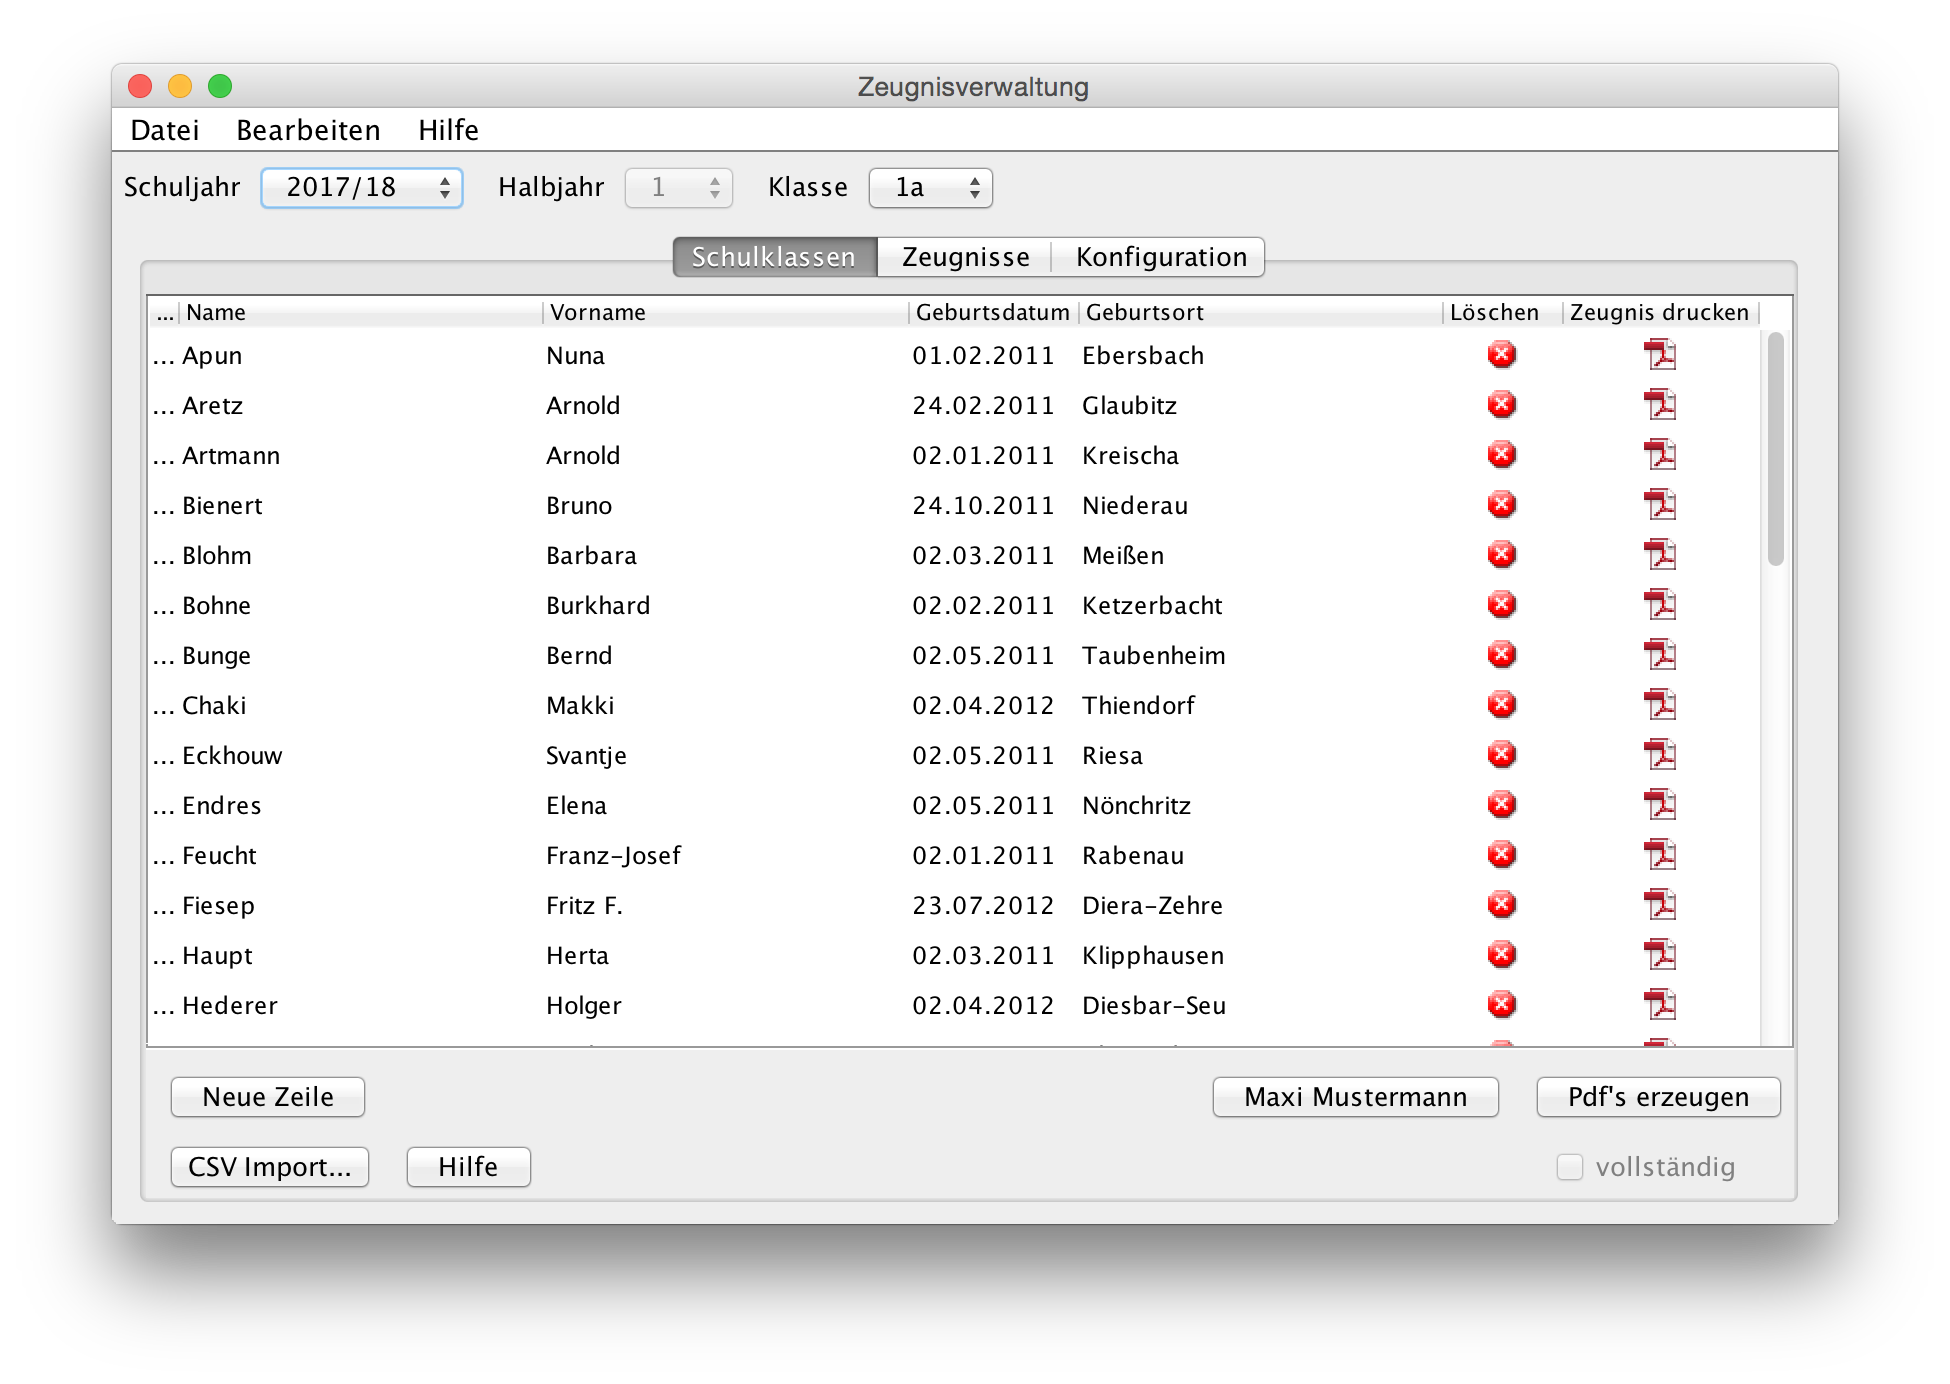
\includegraphics[width=1.0\textwidth]{Schulklassen}}
\caption{Eingabe der Schüler}
\label{fig:Schulklassen}
\end{figure}

Wenn alle Zeugnisse für diese Klasse vollständig bearbeitet wurden und in keinem mehr der Initialwert vorhanden ist, wird rechts unten angezeigt, ob die Schulklasse vollständig ausgefüllt ist.
Dann können alle PDF--Zeugnisse und auch das Durchschnittszeugnis sinnvoll generiert werden\footnote{Man kann die PDF--Zeugnisse natürlich auch unvollständig generieren lassen. Die Anzeige dient nur als Hilfestellung.}.

Im unteren rechten Bereich findet man auch eine Checkbox für das Druckdatum und ein Feld für das Druckdatum.
Wenn diese Checkbox selektiert ist, wird bei der Generierung der PDF--Zeugnisse nicht das aktuelle Datum genommen, sondern das Datum, was in dieses Feld eingetragen wurde.
Dieses Datum wird nicht in der Datenbank gespeichert und bei einem Neustart des Programmes ist das Feld wieder leer und die Checkbox nicht selektiert.
Wenn man ein anderes Druckdatum als das Generierungsdatum erzeugen möchte, so muss man also vor der Generierung der Zeugnisse (einzeln oder alle) diese Checkbox selektieren und das Druckdatum dort eintragen\footnote{Bleibt das Datumsfeld bei selektierter Checkbox leer, so wird eine gepunktete Linie für das handschriftlich zu erzeugende Datum gedruckt.}.

\subsubsection{Batch--Import von Schülern}
Es besteht die Möglichkeit, Schülerlisten über einen Batch--Import in das Programm einzulesen.
Dazu dient der Button \framebox{CSV-Import}. Drückt man ihn, kann man eine Datei auswählen, die die Extension {\ott .csv} oder {\ott .txt} besitzen muss und folgende Komma-getrennte Felder besitzen muss:

\begin{lstlisting}
Vorname, Name, Datum, Geburtsort
\end{lstlisting}

Also z.B.\footnote{Für die technisch Versierten: Wenn Umlaute in den Namen vorhanden sind, sollte das Encoding in der Datei dem Encoding des Betriebssystems entsprechen. Andernfalls werden die Umlaute nicht richtig dargestellt. Das Encoding auf Windows ist oft Windows1252 und auf OSX meist UTF8.}

\begin{lstlisting}
Boris, Becker, 2011-12-31, Leimen
Graf, Steffi, 2012-02-05, Stuttgart
\end{lstlisting}



Dabei muss das Datum in folgenden Format gesetzt sein: {\ott JJJJ-MM-TT} also z.B. {\ott 2011-12-31}.

Die Schüler in dieser Datei werden der aktuellen Schulklasse hinzugefügt.

\subsection{Zeugnis}
Durch Klick auf den Reiter {\ott Zeugnisse} gelangt man in den Eingabemodus für die Zeugnisse.

Hier wählt man zunächst den aktuellen Schüler.
Gegebenenfalls muss man vorher das Schuljahr, das Halbjahr und die Klasse im übergeordneten Bereich vorwählen.
Zu beachten ist, dass es für die Zeugnisse wichtig ist, ob sie für das 1. oder für das 2. Halbjahr gelten sollen, da dies im Ausdruck natürlich gekennzeichnet wird.

Dann werden im linken Bereich der gewünschte Lernbereich ausgewählt, dessen Indikatoren dann in der rechten Tabelle erscheinen.
Für die Lernbereiche Arbeits-- und Sozialverhalten erscheint speziell noch ein Kommentarbereich für freien Text\footnote{5 Zeilen sollten nicht überschritten werden} und eine Auswahlbox unter der Tabelle, in der man die standardisierte Gesamtnote wählen kann. 

Im linken Bereich kann man auch freien Text für die Lernentwicklung und für Bemerkungen angeben. Dabei sind zur Zeit keine Textformatierungen wie fett oder kursiv erlaubt, um ein konsistentes Erscheinungsbild zu erhalten.

Im Bemerkungsfeld werden kurze Bemerkungen eingegeben.
Ist das 2.~Halbjahr vorgewählt worden, so erscheint hier standardmäßig der Text: \emph{Versetzt nach Klasse..{\ott Folgeklasse}}.

Die Länge des Textes speziell die Zeilenanzahl wird z.Z. nicht überprüft\footnote{Achtung: Bei zuvielen Zeilen, kann das Gesamtlayout zerrissen werden!}. Für den Lernentwicklungsbericht sind 3000 Zeichen, für die Bemerkungen sind 1500 Zeichen und für die Kommentare bei dem Arbeits-- und Sozialverhalten sind jeweils 500 Zeichen vorgesehen. Alles darüber hinausgehende wird hart abgeschnitten und wird nicht in der Datenbank gespeichert.

Die gesamten Fehltage und die Fehltage ohne Entschuldigung können darunter angegeben werden.
Dabei sollte beachtet werden, dass im Falle einer widersprüchlichen Angabe wie z.B. Fehltage ohne Entschuldigung sind mehr als gesamte Fehltage, die Fehltage ohne Entschuldigung im Ausdruck korrigiert werden, damit keine peinlichen Zeugnisse erstellt werden. 

Die Bewertungen werden über eine Auswahlbox gewählt, die erscheint, wenn man rechts neben den entsprechenden Indikator klickt. Für die Indikatoren der Lernbereiche \emph{Arbeits-- und Sozialverhalten} werden die Bewertungen in Textform ausgewählt. Für den Rest der Bewertungen werden teilweise gefüllte Kreise bereitgestellt.

Für jeden Lernbereich müssen so die Indikatoren bewertet werden.
Ist zu jedem Indikator eine Bewertung erfolgt (Bewertungsfeld ist nicht leer) erscheint ein Häkchen neben dem Schülernamen, der anzeigt, dass das Zeugnis nun komplett ist und gedruckt werden kann.

Abbildung~\ref{fig:Zeugnisse} auf Seite~\pageref{fig:Zeugnisse} zeigt die Eingabe der Bewertungen für die Lernbereiche \emph{Arbeits-- und Sozialverhalten}.
Abbildung~\ref{fig:Zeugnisse2} auf Seite~\pageref{fig:Zeugnisse2} zeigt die Eingabe der Bewertungen für die anderen Lernbereiche.

\begin{figure}[H]
\centering
\centerline{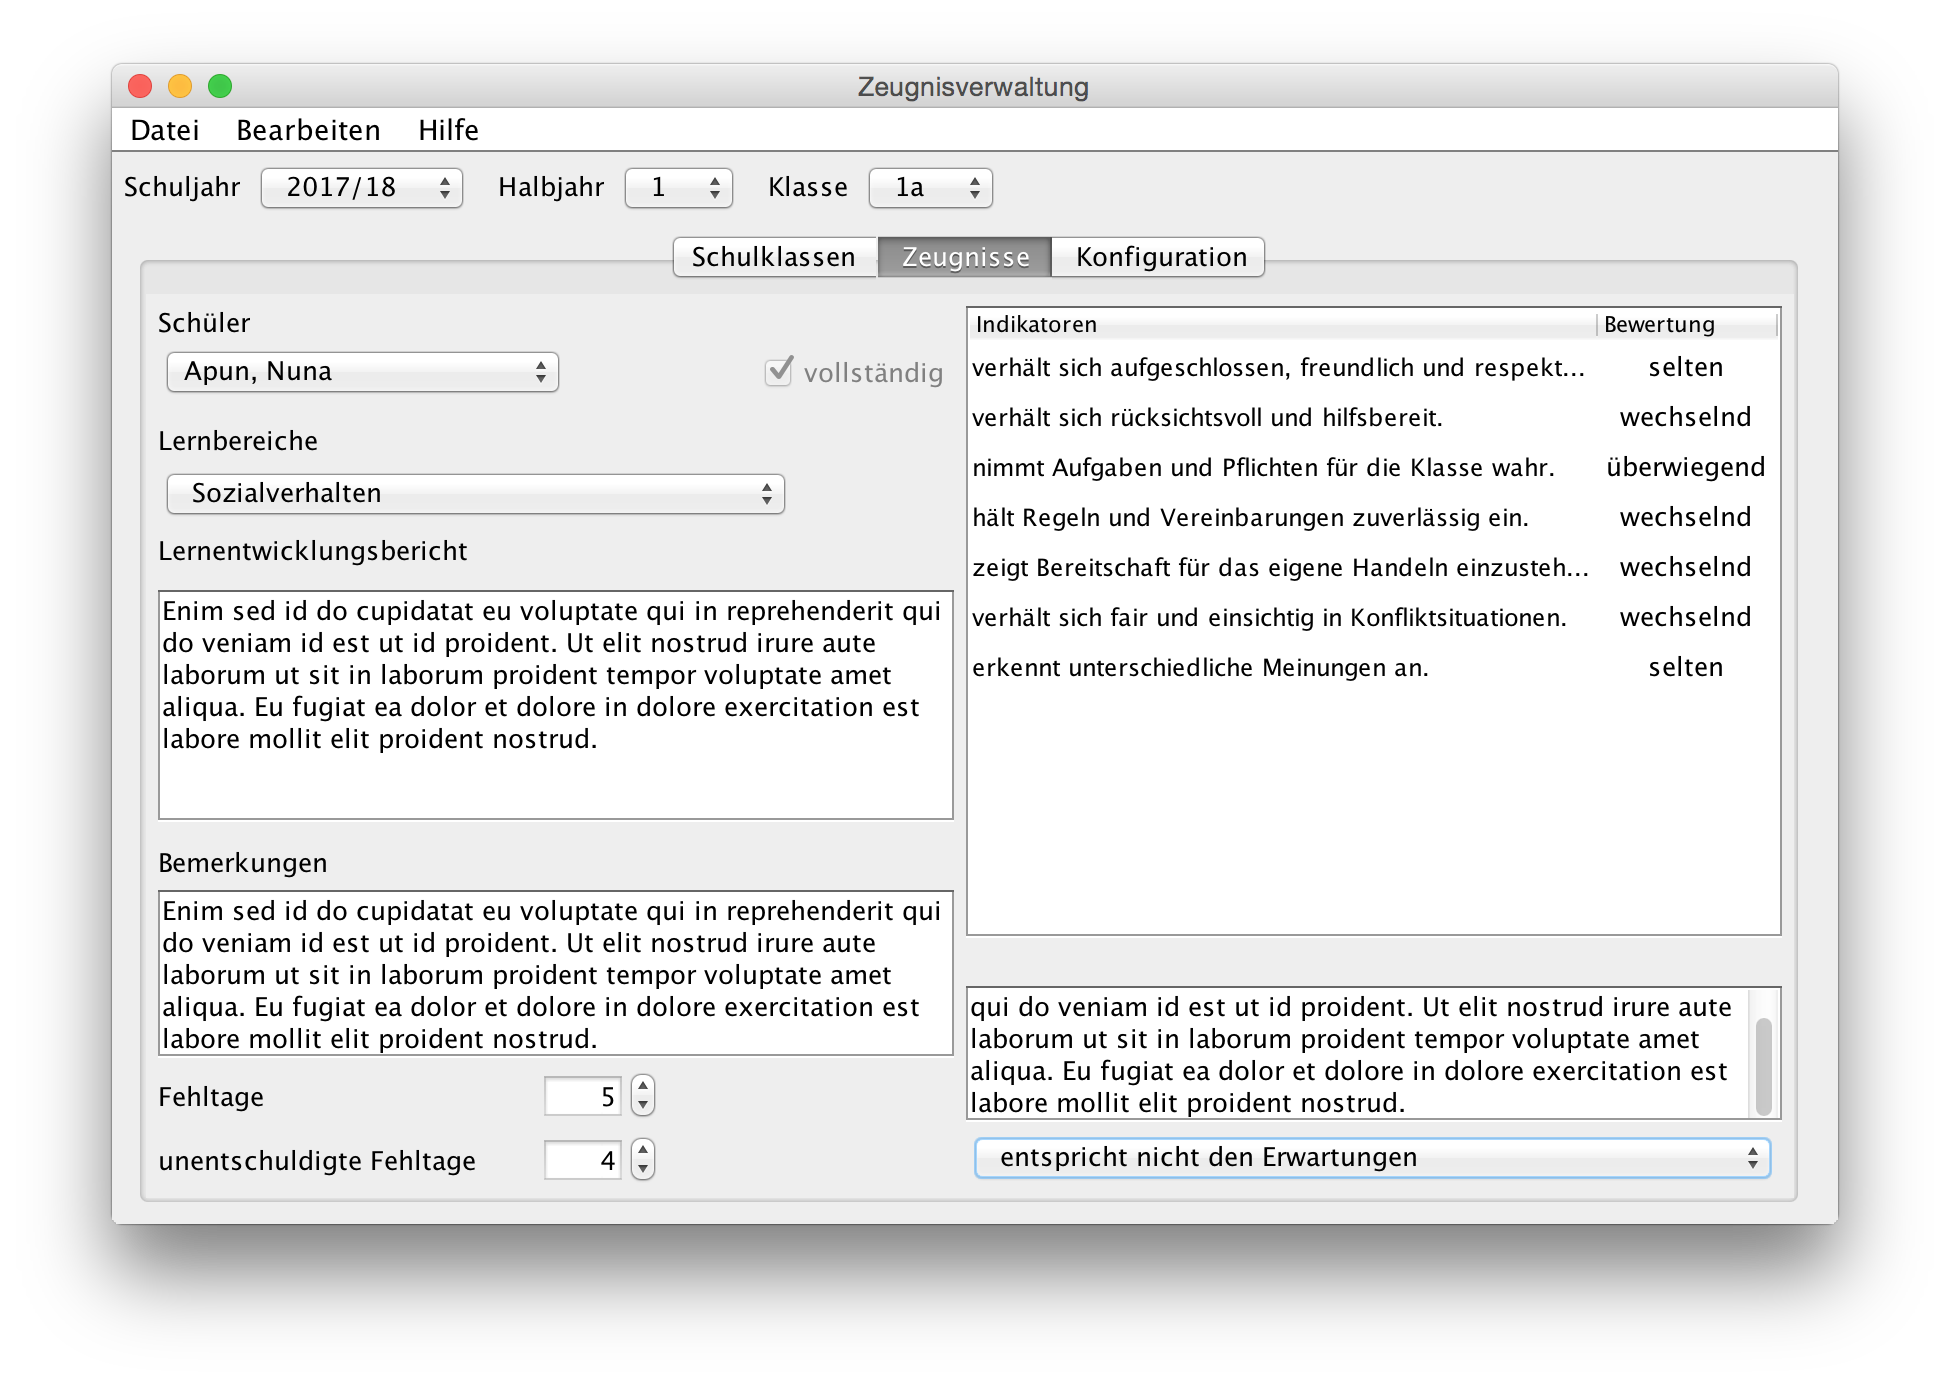
\includegraphics[width=1.0\textwidth]{Zeugnisse.png}}
\caption{Ausfüllen der Zeugnisse (Arbeits-- und Sozialverhalten)}
\label{fig:Zeugnisse}
\end{figure}

\begin{figure}[H]
\centering
\centerline{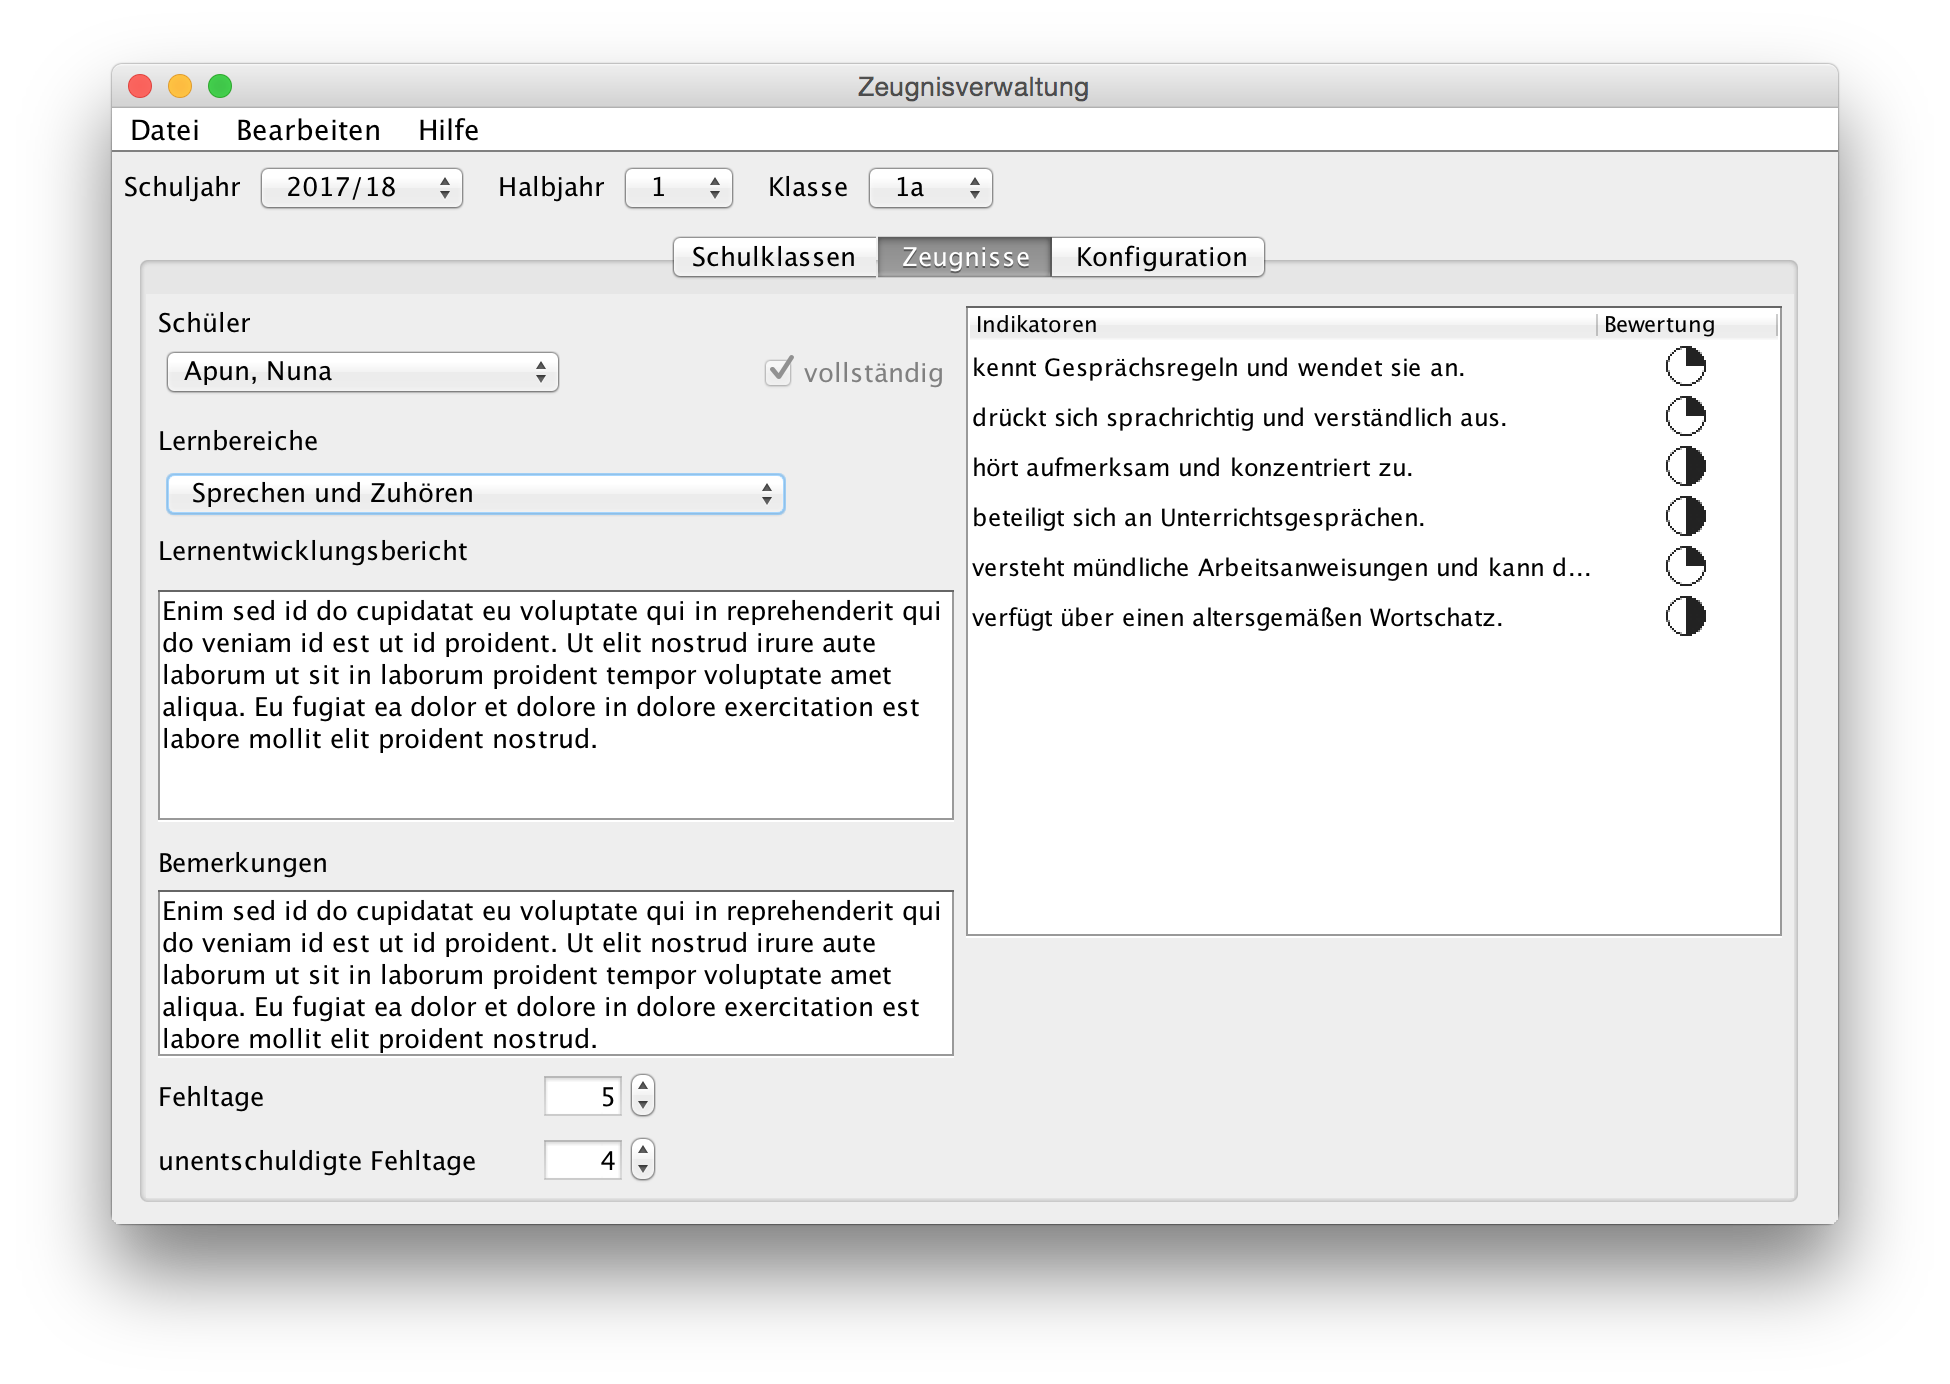
\includegraphics[width=1.0\textwidth]{Zeugnisse2}}
\caption{Ausfüllen der Zeugnisse (andere Lernbereiche)}
\label{fig:Zeugnisse2}
\end{figure}

\subsection{Konfiguration}
\begin{figure}[H]
\centering
\centerline{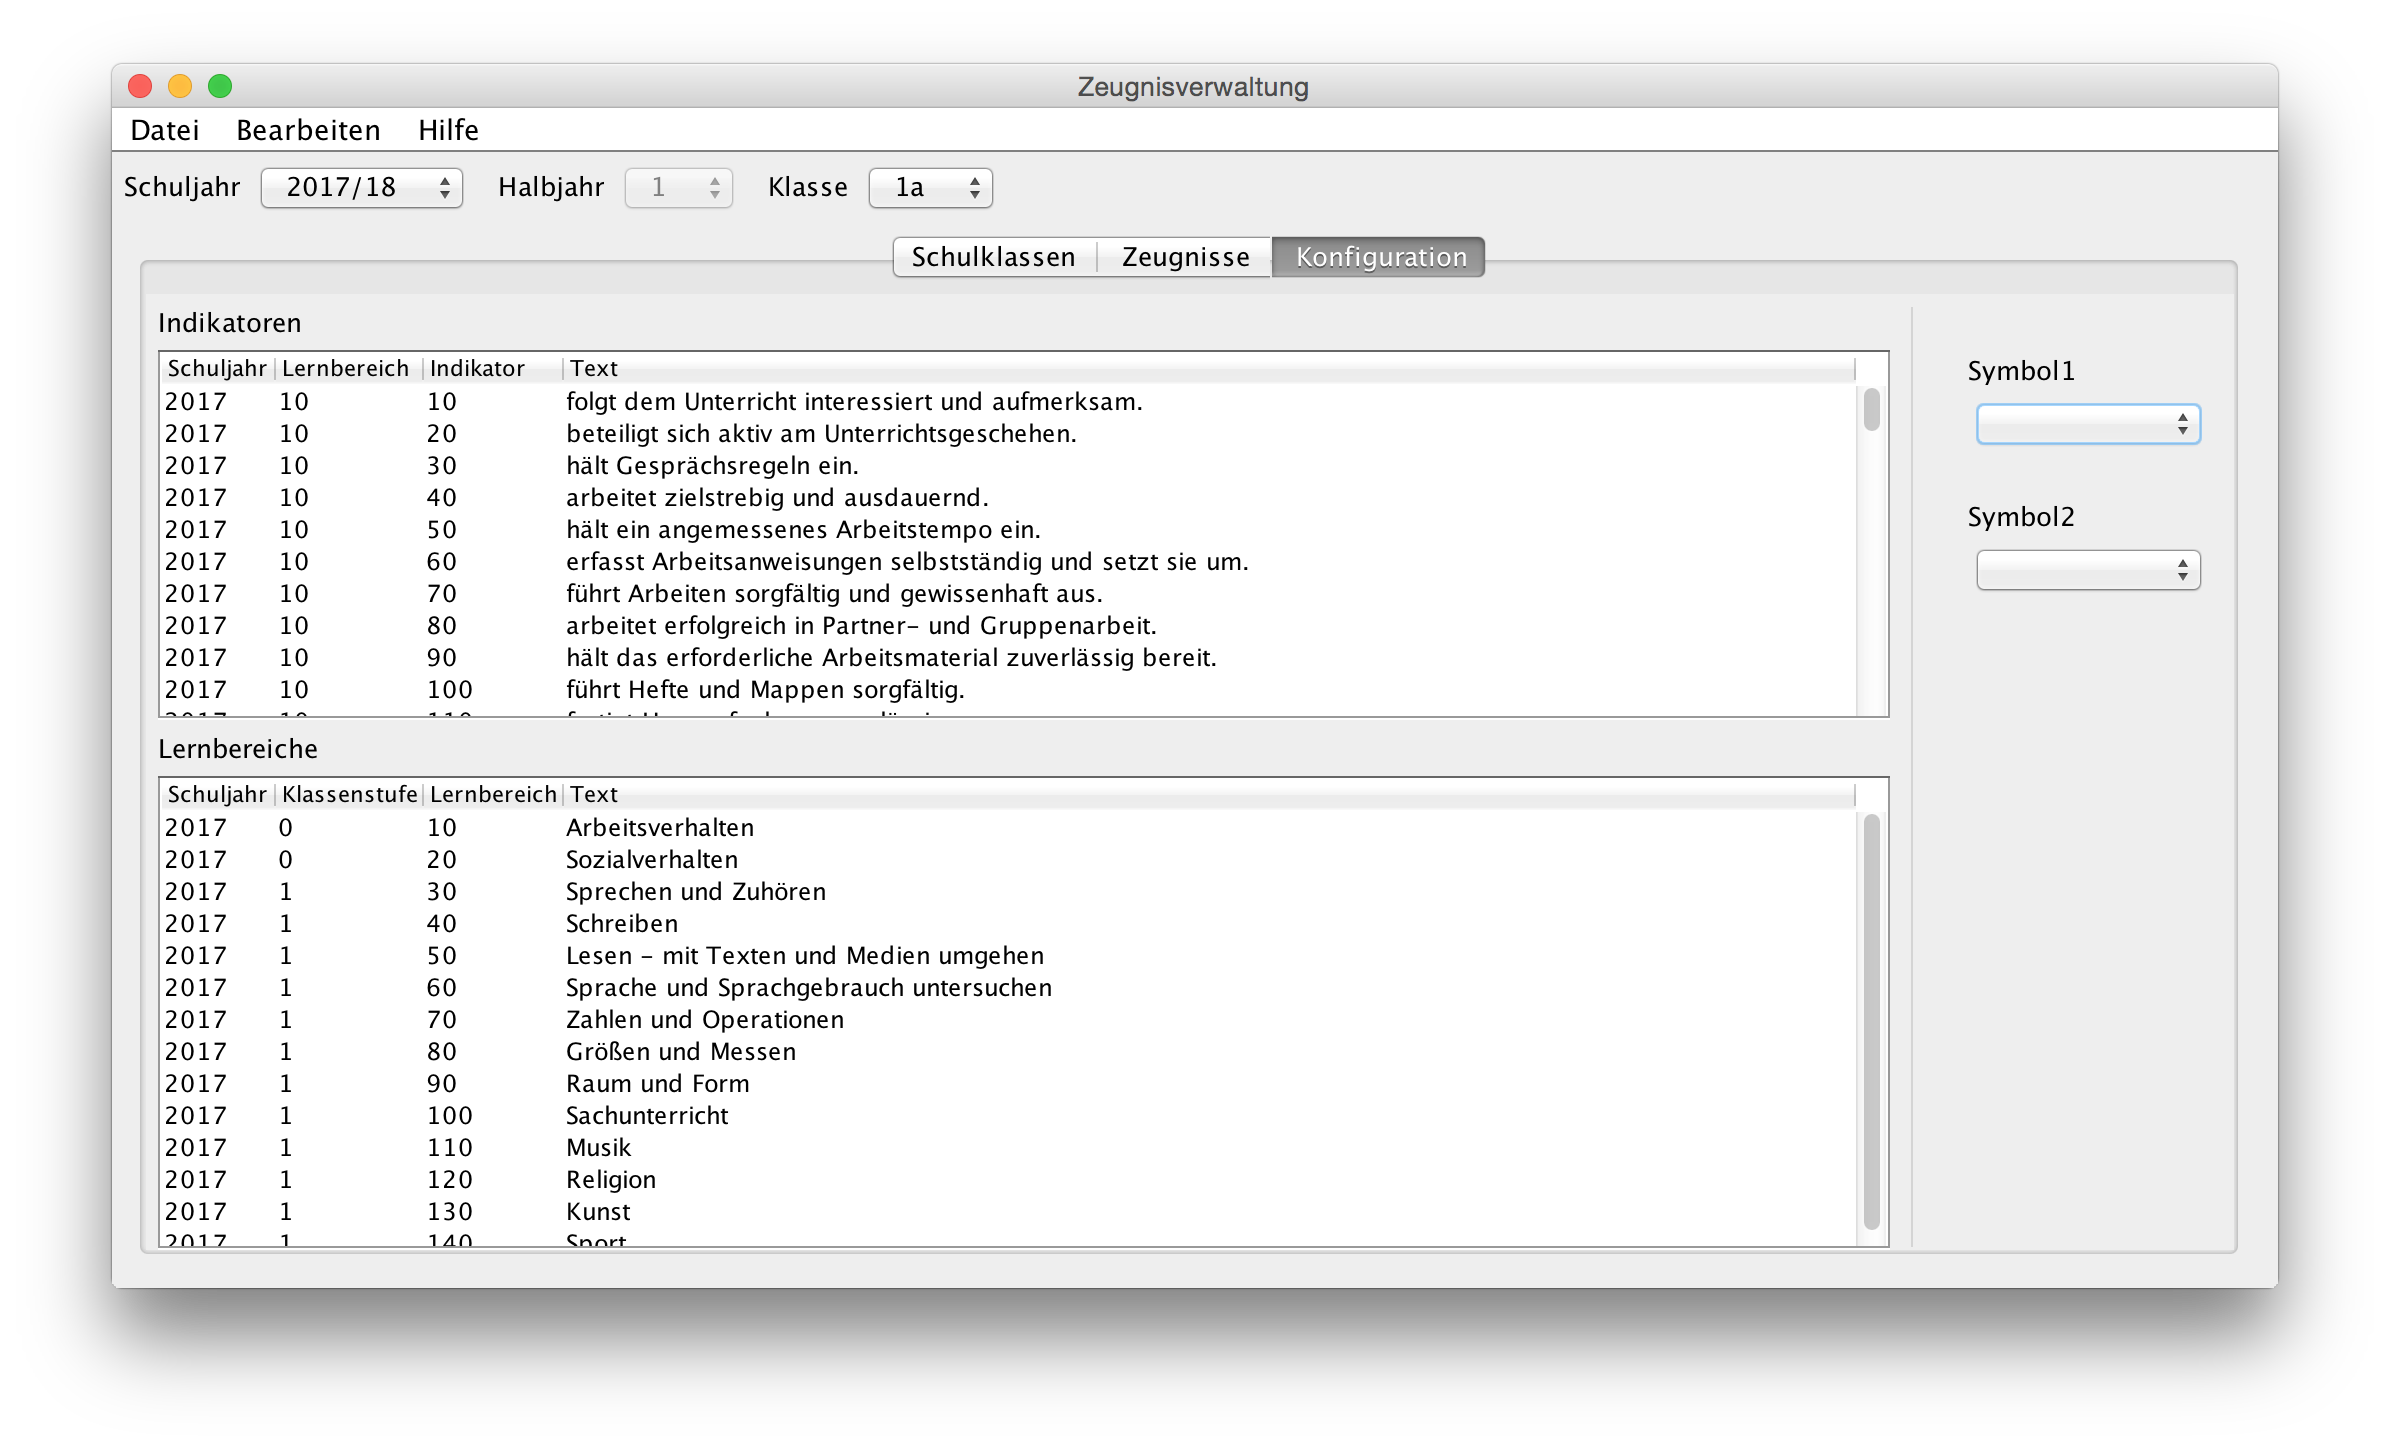
\includegraphics[width=1.0\textwidth]{Konfiguration}}
\caption{Verändern der Indikatoren und Zeugnissymbole}
\label{fig:Konfiguration}
\end{figure}
\subsubsection{Symbole}
Die Symbole, die im Ausdruck bei den Indikatoren erscheinen können hier verändert werden.

\emph{Symbol1} ist das Symbol, dass beim Arbeits-- und Sozialverhalten verwendet wird. \emph{Symbol2} ist das Symbol, dass bei den anderen Lernbereichen verwendet wird.

Änderungen, die hier gemacht werden, werden auch in der {\ott config.properties}--Datei abgespeichert und stehen beim nächsten Aufruf des Programms wieder zur Verfügung.

\begin{table}[H]
\begin{center}
\begin{tabular}{|l|c|}
\hline
Symbolnummer & Bild \\
\hline
Symbol 1& 
\includegraphics[width=5mm]{img01.png} \\
Symbol 2& 
\includegraphics[width=5mm]{img02.png} \\
Symbol 3& 
\includegraphics[width=5mm]{img03.png} \\
Symbol 4& 
\includegraphics[width=5mm]{img04.png} \\
Symbol 5& 
\includegraphics[width=5mm]{img05.png} \\
Symbol 6& 
\includegraphics[width=5mm]{img06.png} \\
Symbol 7& 
\includegraphics[width=5mm]{img07.png} \\
Symbol 8& 
\includegraphics[width=5mm]{img08.png} \\
Symbol 9& 
\includegraphics[width=5mm]{img09.png} \\
Symbol 10& 
\includegraphics[width=5mm]{img10.png} \\
Symbol 11& 
\includegraphics[width=5mm]{img11.png} \\
Symbol 12& 
\includegraphics[width=5mm]{img12.png} \\
Symbol 13& 
\includegraphics[width=5mm]{img13.png} \\
Symbol 14& 
\includegraphics[width=5mm]{img14.png} \\
\hline
\end{tabular}
\caption{Tabelle der Symbole}
\end{center}
\end{table}

\subsubsection{Indikatoren}
Sollte es mal notwendig sein, die Formulierungen der Indikatoren zu verändern, ist dies hier möglich.
Da diese Formulierungen aber von allen Zeugnissen mit den übergeorneten Parametern verwendet werden, sollte man dies mit Vorsicht benutzen.

Da man hier direkt in die zugrunde liegende Datenbank schreibt, ist es nötig, zu verstehen, wie die Daten organisiert sind.

Die untere angezeigte Tabelle (Lernbereich) dient nur zur Übersicht und kann nicht editiert werden.
Es können also keine neuen Lernbereiche erzeugt, vorhandene verändert oder gelöscht werden, da dies weitreichende Folgen auch für den Ausdruck hätte.

Für jedes Schuljahr und für jede Klassenstufe gibt es eigene Lernbereiche, die einmal in Textform und zum anderen als Nummer angesprochen werden können.

Diese Tabelle ist deshalb hier aufgeführt, damit man weiss, für welchen Lernbereich man gegebenenfalls die Indikatoren verändern möchte und nicht versehentlich die gleichlautenden Indikatoren für andere Klassenstufen oder Schuljahre verändert. Der Lernbereich \emph{Schreiben} für das Schuljahr 2017/18 und die erste Klassenstufe hat z.B. die Nummer $40$.
Der Lernbereich \emph{Schreiben} für das Schuljahr 2017/18 und die vierte Klassenstufe hat z.B. die Nummer $430$; indem man oben die entsprechende Klasse einstellt kommt man zu diesen Werten.

In der oberen Tabelle kann man nun gezielt den Text der Indikatoren für diesen Lernbereich verändern. Sobald man dort das editierte Feld verlässt, wird die Änderung in die Datenbank übernommen und steht beim nächsten Ausfüllen oder Anzeigen des Zeugnisses zur Verfügung.

Indikatoren, die keinen Text besitzen und die später ein leeres Bewertungsfeld besitzen, werden im Ausdruck des Zeugnisses nicht berücksichtigt.

Für alle Lernbereiche ausser \emph{Arbeits-- und Sozialverhalten} gibt es immer ein leeres Indikatorfeld, für Erweiterungen, so dass mindestens ein weiterer Indikator hinzugefügt werden kann\footnote{In Folgeversionen wird das eventuell erweitert.}.

Abbildung~\ref{fig:Konfiguration} auf Seite~\pageref{fig:Konfiguration} zeigt die Eingabe der Bewertungen für die anderen Lernbereiche.

\subsubsection{Änderungen in {\ott config.properties}}
\label{configKlassen}
In der Konfigurationsdatei {\ott config.properties} können einige Werte des Programms konfiguriert werden, die dann beim nächsten Start des Programms initial verwendet werden.

Zum einen sind das die Symbole in den ausgedruckten Zeugnisse, die auch im Programm verändert werden können.
Wichtig ist hier, dass zur Zeit nur 14 Symbole zur Verfügung stehen (1\dots14). Zahlen, die nicht in diesem Bereich liegen, könnten zu Fehlern führen.

Zum anderen können hier die Klassen eingegeben werden, die verwendet werden sollen (1a,1b,2a,\dots).
Zur Zeit sollten die Klassen in diesem Format eingegeben werden, da das Programm intern davon ausgeht, dass die erste Stelle die Klassenstufe angibt und die zweite Stelle ein Buchstabe ist.

\subsection{Schnittstellen}
Das Programm besitzt keine Schnittstellen zu externen Programmen. Es ist zur Zeit kein Import oder Export möglich.
Die einzige Ausgabe ist das Zeugnis selbst in einem PDF--Format.

\section{Neues Schuljahr}
Im Menü {\ott Bearbeiten} kann ein neues Schuljahr angelegt werden. Dazu werden alle vorhandenen Grunddaten (Lernbereiche und Indikatoren) auf ein neues Schuljahr übertragen.
Im neuen Schuljahr werden die Schülerlisten von den vorherigen Klassen übernommen:
Schüler aus der Klasse 1a werden im neuen Schuljahr in die Klasse 2a kopiert usw. .
Die pro Schüler generierten Halbjahreszeugnisse sind zunächst leer.

Ein neues Schuljahr kann nur in der 2.~Hälfte des Schuljahres angelegt werden.
Also im Schuljahr 2017/18 kann erst im Jahr 2018 ein neues Schuljahr 2018/19 angelegt werden. Weitere Schuljahre können nun erst wieder im Jahre 2019 angelegt werden. Schuljahre können nicht wieder gelöscht werden.
Die Indikatoren und Lernbereiche werden immer aus dem \emph{aktuellen} Schuljahr in das neue Schuljahr kopiert; das ist besonders wichtig, wenn die Indikatoren vorher manuell editiert wurden.

\section{Durchschnitt}
Bei den Schulklassen gibt es noch einen Button mit der Aufschrift \emph{Maxi Mustermann}.
Wenn man diesen Button drückt, wird im aktuellen Ordner für die Zeugnisse ein Zeugnis mit Durchschnittswerten aus der Klasse angelegt. Wenn kein Schüler in der Klasse vorhanden ist, wird keine Datei erzeugt.

Folgende Werte werden dann in das Zeugnis eingetragen:

\begin{center}
\begin{tabular}{rl}
\hline
\emph{Name}                    	& Mustermann\\
\emph{Vorname} 					& Maxi\\
\emph{Geburtsdatum} 			& aktuelles Datum\\
\emph{Geburtsort} 				& der häufigste Geburtsort\\
\emph{Fehltage} 				& arithmetisches Mittel aller Fehltage\\
\emph{Fehltage ohne Entsch.} 	& arithmetisches Mittel aller Fehltage ohne Entschuldigung\\
\emph{Lernentwicklung} 			& dieser Erklärungstext\\
\emph{Note Arbeitsverhalten} 	& arithmetisches Mittel aller Noten\\
\emph{Note Sozialverhalten} 	& arithmetisches Mittel aller Noten\\
\emph{Bewertungen Lernbereiche} & arithmetische Mittel der Bewertungen\\
\hline
\end{tabular}
\end{center}


Der Name \emph{Maxi Mustermann} ist nur ein Default Name. Falls noch keine {\ott config.properties} angelegt wurde, wird dieser als Standardname verwendet. Sobald die Datei {\ott config.properties} 
erzeugt wurde, kann man in der {\ott config.properties} den Namen verändern:

\begin{itemize}
\setlength{\itemindent}{3.5cm}
\item[sName] Nachname
\item[sVorname] Vorname
\end{itemize}

Der neue Name erscheint dann auf dem Button und in dem entsprechenden Durchschnittszeugnis.
\section{Speicherorte}
Wenn die Zeugnisse abgespeichert werden, werden automatisch Ordner im Verzeichnis des Programms angelegt, in denen das Schuljahr, das Halbjahr und die Schulklasse kodiert sind, als z.B.
{\ott\normalfont\bfseries 201611a} für das Schuljahr 2016/17, das erste Halbjahr und die Klasse 1a oder z.B. {\ott\normalfont\bfseries 201724b}
für das Schuljahr 2017/18, das 2.~Halbjahr und die Klasse 4b.
Wann immer ein Zeugnis generiert wird (auch zur Anzeige) werden diese Zeugnisse in diesen Ordner gespeichert. Alte Zeugnisse werden automatisch überschrieben.

Im Schulklassen--Reiter gibt es einen Button, der für alle dort aufgeführten Schüler ein Zeugnis generiert und in den entsprechenden Ordner abspeichert.

\section{Beispielausdruck für 4 Schuljahre}
Hier folgt ein Beispielausdruck aller Zeugnisses (1.-- 4. Jahrgang), das vollständig ausgefüllt wurde.


\includepdf[pages=-]{BeckerBoris.pdf}

\includepdf[pages=-]{GrafSteffi.pdf}

\includepdf[pages=-]{MerkelAngela.pdf}

\includepdf[pages=-]{FourthColin.pdf}


\section{Schlussbemerkung}
Dieses Programm ist die erste Version und kann daher noch einige Fehler enthalten.
Fehler sollten daher den Autoren per Email gemeldet werden.

\end{document}